\section{Introduction}
Terrain-adaptive locomotion is essential for enhancing the mobility of legged robots and moving beyond blind walking strategies \citep{di2018dynamic,kim2019highly, zhou2022momentum}. Many existing methods achieve terrain adaptability by adjusting footholds around a nominal trajectory in real time \citep{fankhauser2018robust,grandia2023perceptive}. To further boost traversability, some approaches have explored variable gait patterns. In \citep{Park2015OnlinePF, kim2020vision,gilroy2021autonomous}, jumping motions are precomputed offline and triggered heuristically upon detecting obstacles. Other methods embed gait switching—such as transitions from walking to jumping—within simplified dynamics models during trajectory sampling \citep{norby2020fast}, or rely on pre-trained classifiers to assess feasibility \citep{chignoli2022rapid}. However, despite the importance of safety in high-risk settings such as disaster zones and construction sites, relatively few works address formal safety guarantees for agile, variable-gait locomotion \citep{zhao2022reactive,shamsah2023integrated} that fully account for the robot's physical limitations.

%%%% Fig.2 System architecture %%%%
\begin{figure}[t]
    \centering
    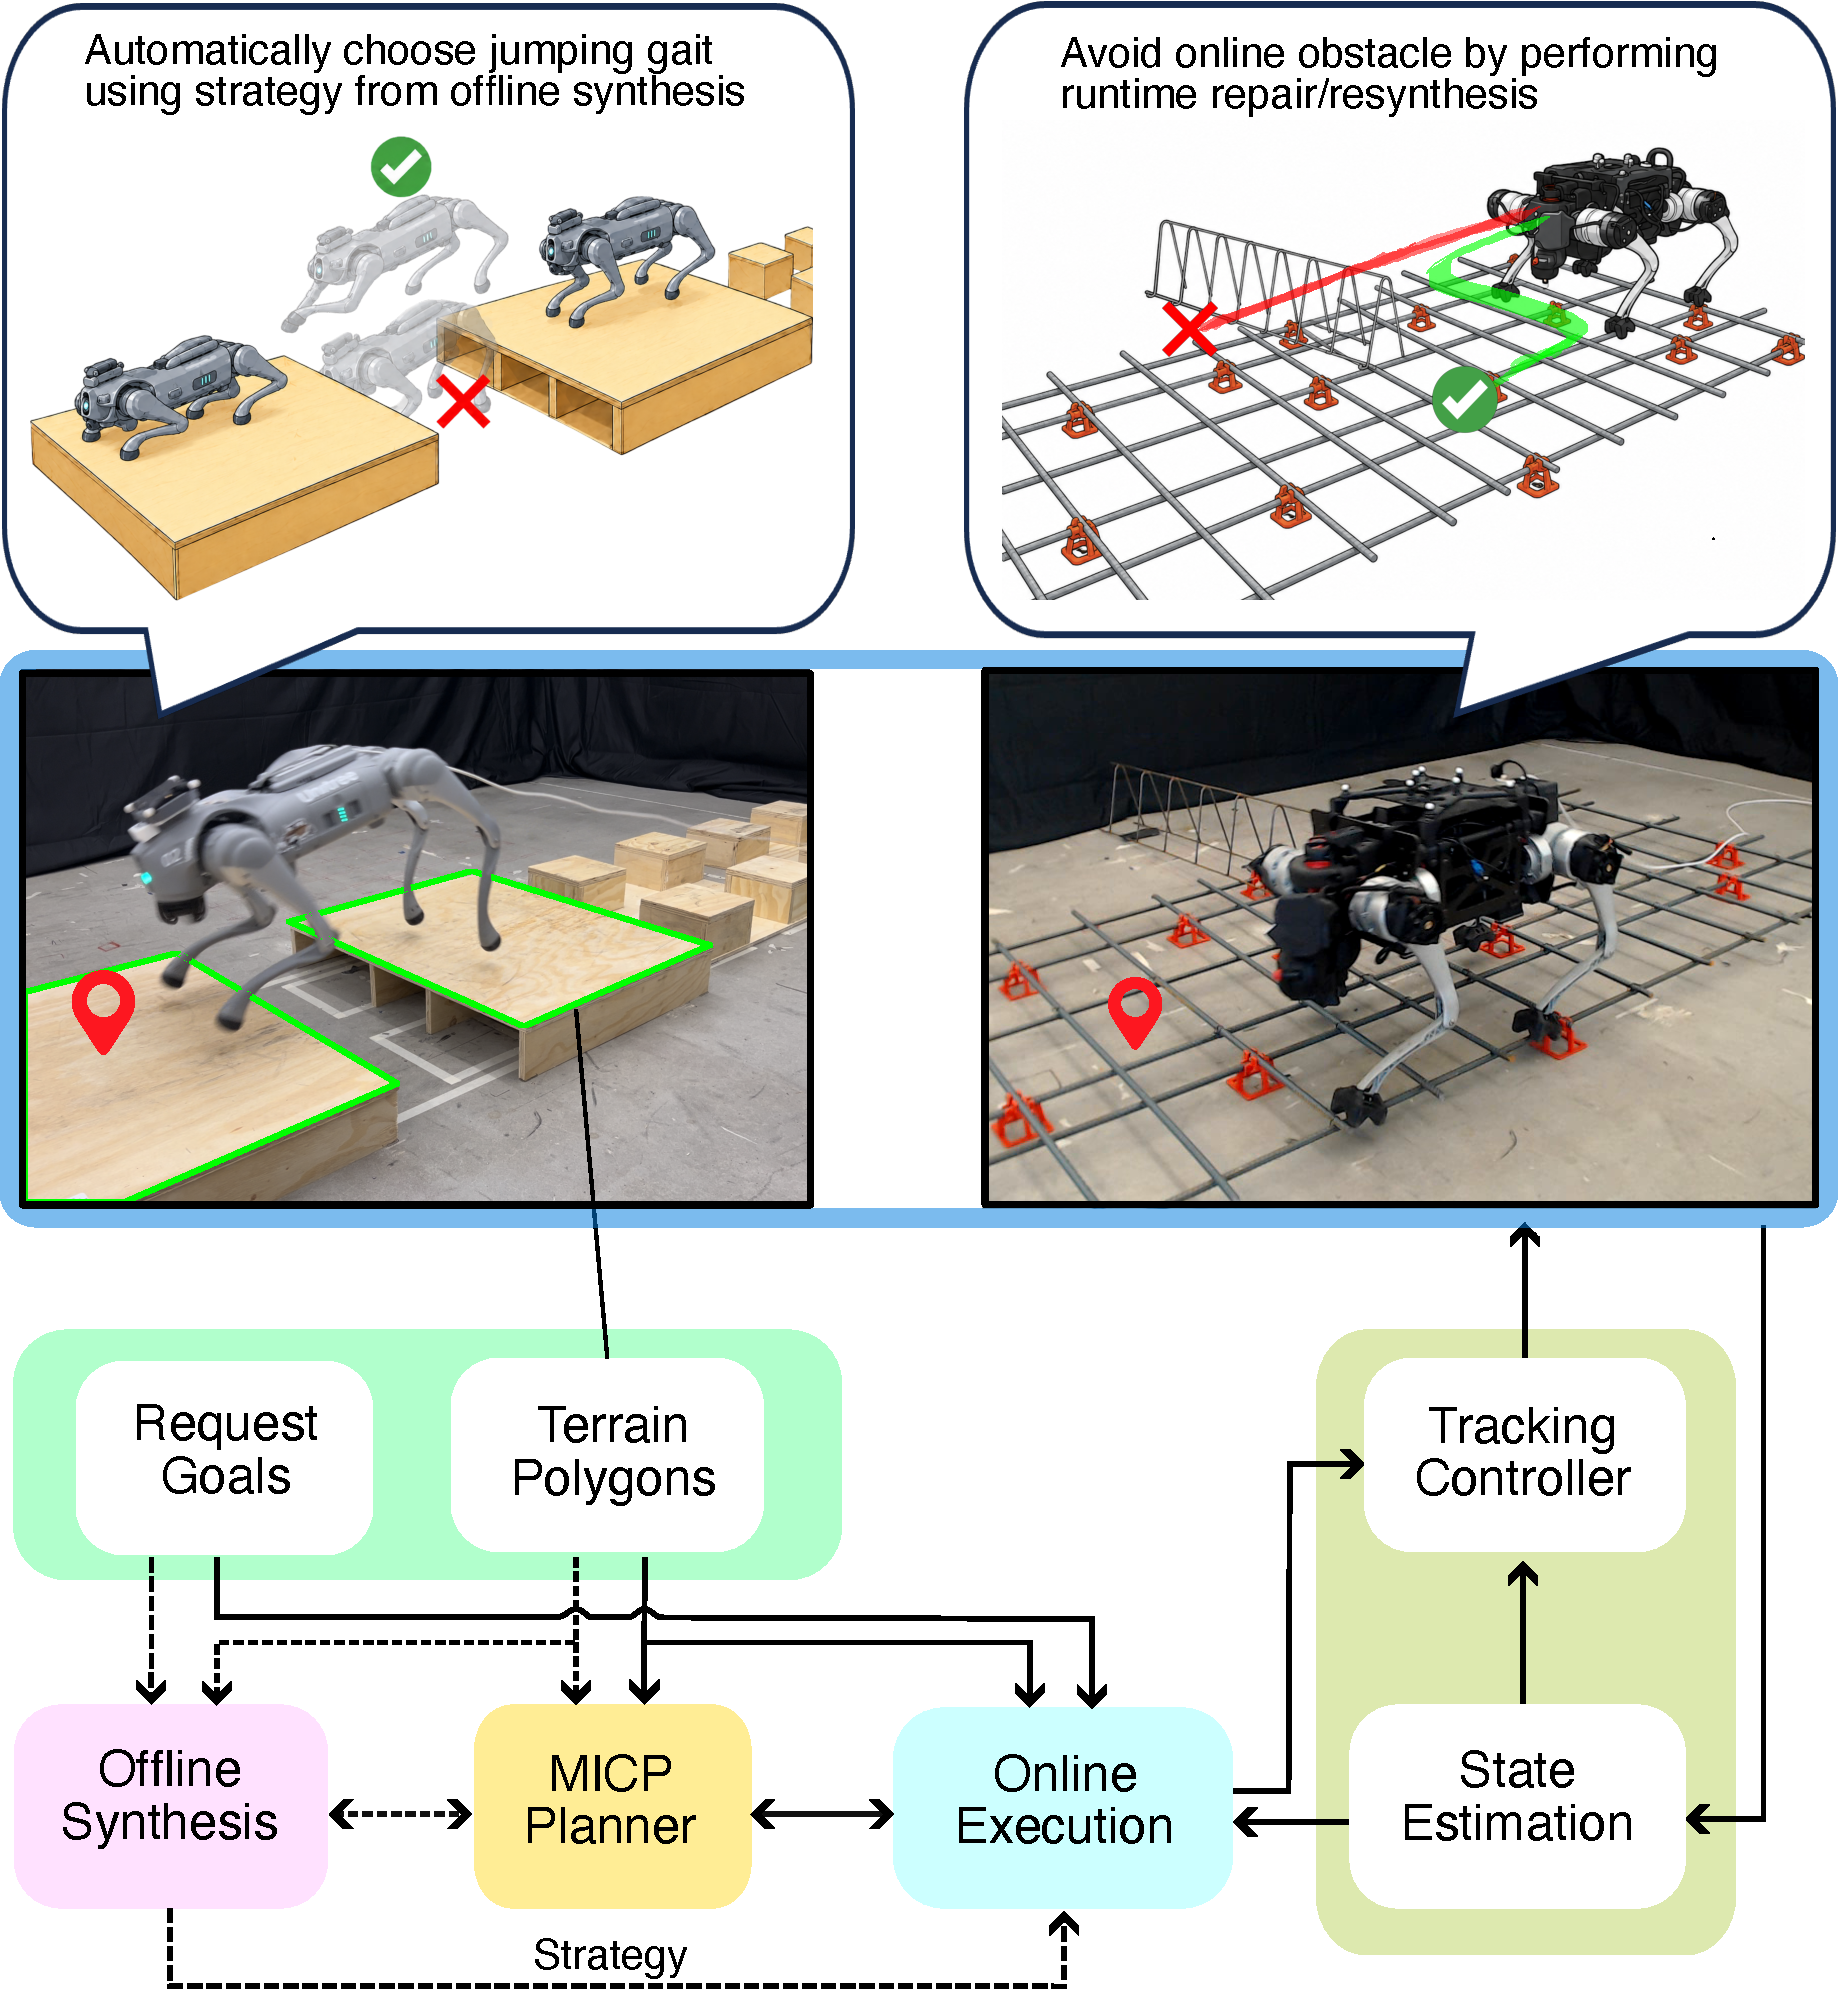
\includegraphics[width=1\linewidth]{system_diagram_v4.pdf}
    \caption{System architecture overview. The solid lines indicate online communication, while dashed lines represent offline processes.
    The request goals in the offline phase are user-defined, while those in the online phase are provided by a global planner based on the global goal.
    }
    \label{fig:system_diagram}
\end{figure}
%%%%%%%%%%%%%%%%%%%%%%%%%%%%%%%%%%%

Mixed-integer programming (MIP)-based methods \citep{valenzuela2016mixed,shirai2022simultaneous} model both contact state and contact surface selection for each leg and timestep as binary decision variables. This allows them to explicitly capture the interaction between terrain geometry and the robot's kinematic and dynamic constraints \citep{deits2014footstep}. When dynamics and constraints are suitably relaxed, the resulting convex approximation (MICP) provides a global certificate of feasibility upon convergence \citep{dai2019global}, making it a powerful tool for formally assessing locomotion viability.
However, the computational demands of MIP-based approaches scale poorly with increased terrain complexity and longer planning horizons, posing a major hurdle for real-time applications. To mitigate this, various simplifications have been proposed, such as fixing contact sequences \citep{ding2020kinodynamic,fey20243d}, constraining timing \citep{ponton2016convex,risbourg2022real,acosta2023bipedal}, or limiting the number of footsteps \citep{aceituno2017simultaneous}. Despite these efforts, scalability remains a challenge in cluttered environments with various terrain segments and features.

To simplify navigation across complex terrains, one effective strategy is to decompose long-horizon, global tasks into a sequence of localized, robot-centric environments centered around intermediate waypoints \citep{fankhauser2018robust}. Despite this simplification, the associated MIP formulation still faces computational challenges, as it must account for all nearby terrain elements.
To address this, we discretize the local environment and constrain each MIP to solving only a single discrete transition at a time. These discrete transitions are then composed using a Linear Temporal Logic (LTL)-based reactive synthesis framework \citep{bloem2012synthesis}, which enables us to systematically construct a correct-by-construction strategy that guides the robot through local decisions toward achieving its intermediate goals.
\revised{For readers unfamiliar with formal methods, LTL is a logic for expressing temporal properties of system behaviors using operators such as ``always,'' ``eventually,'' and ``until''~\citep{piterman2006synthesis,bloem2012synthesis}; reactive synthesis automatically constructs a controller (named as a \emph{strategy automaton} in this paper) that satisfies an LTL specification against any admissible environment behavior, providing correct-by-construction guarantees at the symbolic level.}

In this work, we present an integrated planning framework that unifies reactive synthesis with MIP-based optimization to enable legged robots to respond safely and efficiently to \revised{unforeseen terrain configurations revealed at runtime}. We abstract both the continuous robot states and local environmental context into symbolic representations, allowing the robot to make high-level decisions in real time for negotiating complex obstacles such as large gaps or cluttered terrain (see Fig.~\ref{fig:system_diagram}). Each symbolic transition is validated through an MICP to ensure the physical feasibility of the locomotion process. This architecture not only connects high-level symbolic reasoning with low-level dynamic feasibility, but also mitigates the computational challenges of solving long-horizon MICP problems.
By leveraging guidance from the LTL-based symbolic planner, each MICP instance only needs to handle short horizons and a limited set of terrain features, which substantially reduces computational load.
The framework is two-stage: in the offline synthesis stage, we employ \textit{gait-free} MICP formulations that jointly optimize over contact mode and foothold placement to precompute a diverse set of locomotion skills for symbolic transitions. During online deployment, we switch to lightweight \textit{gait-fixed} MICP formulations using these precomputed gaits, enabling real-time generation of physically consistent motions with real-world terrain data.

\revised{The two-stage architecture exposes two scalability challenges that we address with two complementary mechanisms. First, the full task specification has a state space that grows exponentially with the number of variables encoding the surrounding terrains, so direct synthesis is computationally impractical~\citep{bloem2012synthesis}; to address this, we propose a high-level manager that fixes the local terrain and goal information and only retains the skills needed for the current local environment, yielding an $80.9$--$90.1\%$ reduction in the symbolic variable count in our experiments. Second, gait-free MICP---used to certify dynamic feasibility---is itself computationally expensive; we therefore use a symbolic repair process that suggests only the missing transitions whose feasibility must be checked, yielding a $71.6$--$97.6\%$ reduction in costly gait-free MICP solves relative to exhaustive enumeration. During online execution, the gait-fixed MICP is re-solved against the actual perceived terrain to generate a new nominal trajectory, and runtime symbolic repair handles any unforeseen terrain that the offline phase did not cover.}

\revised{Closing the loop between this synthesis-MICP framework and a real robot poses two practical challenges that we address through two additional online-execution mechanisms. (i) Online MICP solve times are inherently variable, ranging from hundreds of milliseconds to several seconds, and can exceed the trajectory horizon used by the tracking controller. We propose a \emph{delay-aware coordination} scheme that asynchronously appends or stalls the tracking trajectory based on a formal two-case analysis of the per-transition timing budget; without it, the closed loop between the discrete strategy automaton and the continuous-time tracker is ill-defined under bounded solve time. (ii) The online MICP tends to become infeasible when the offline-checked target pose mismatches the actual terrain. We add a lightweight, zero-horizon \emph{kinematic-feasibility re-targeting} step that pre-checks and adjusts the desired pose at each transition, decoupling offline pose specification from online terrain geometry; the same online MICP is also augmented with additional collision-avoidance constraints for swing-foot clearance during a transition. Together with the offline scalability machinery, these mechanisms make the framework end-to-end deployable, which we validate on two robot hardware platforms and benchmark against both a pure-MIP planner and a heuristic foothold planner.}

The proposed framework remains flexible and modular---it can be driven by commands from a higher-level planner \citep{wermelinger2016navigation, fernbach2017kinodynamic,norby2020fast,chignoli2022rapid,liao2023walking,feng2023gpf} or directly from a user, and it easily accommodates new behaviors by expanding the symbolic transition set.

The main contributions of this work are summarized as follows:
\begin{itemize}
    \item \textbf{Integrated reactive-synthesis and MICP framework for terrain-adaptive locomotion.}
    Symbolic-level guidance limits the planning horizon and the number of terrain features any single MICP must consider, bridging high-level symbolic reasoning with low-level physical feasibility.

    \item \textbf{Scalable offline synthesis via a high-level manager and symbolic repair with dynamic feasibility checks.}
    The high-level manager reduces the symbolic state space by $80.9$--$90.1\%$, and symbolic repair, equipped with dynamic feasibility checks via gait-free MICP, generates only the necessary skills---reducing costly gait-free MICP solves by $71.6$--$97.6\%$ versus exhaustive enumeration.

    \item \textbf{Online execution module that bridges offline synthesis and real-world deployment.}
    The module re-solves a gait-fixed MICP against the actual perceived terrain at each symbolic transition, with \revised{delay-aware coordination between the strategy automaton and the tracking controller, online kinematic-feasibility re-targeting of the desired pose, and additional collision-avoidance constraints in the online MICP. Runtime symbolic repair handles previously unseen scenarios that were not considered offline.}

    \item \revised{\textbf{Comprehensive experimental validation.} We report simulation across four terrain scenarios with full per-module timing, comparisons against a pure MIP planner and a heuristic foothold planner, hardware deployment of the integrated stack on two robot platforms (Unitree Go2 and SkyMul Chotu), and a feasibility study of yaw orientation as a generalization case study.}
\end{itemize}

A conference version of this work is presented in \citep{zhou2025physically}. Beyond the conference paper, the current article contributes the delay-aware coordination and online re-targeting mechanisms motivated above, full hardware validation of the integrated framework on two robot platforms, systematic benchmarking against a pure-MIP planner and a heuristic foothold planner, a preliminary yaw-extension feasibility study, and substantially expanded preliminaries, related-work survey, and discussion of limitations.


% A conference version of this work is presented in \citep{zhou2025physically}. \revised{Following the IJRR convention for evolved-paper journal extensions, this article restates the framework introduced in the conference version and adds substantial new content. Beyond \citep{zhou2025physically}, the journal-specific contributions are: (i) kinematic-feasibility re-targeting of the robot's desired pose at each transition; (ii) delay-aware coordination between the strategy automaton and the tracking controller, with explicit two-case logic that handles MICP solve-time variability against the NMPC horizon; (iii) collision-region selection with binary variables and swing-foot clearance constraints in the MICP; (iv) full hardware deployment of the integrated stack on two robot platforms; (v) systematic benchmarking against a pure MIP planner and a heuristic foothold planner; (vi) a preliminary feasibility study of yaw orientation as a generalization direction; and (vii) expanded preliminaries, related-work survey, and discussion of limitations.}